\documentclass[tikz]{standalone}
\begin{document}
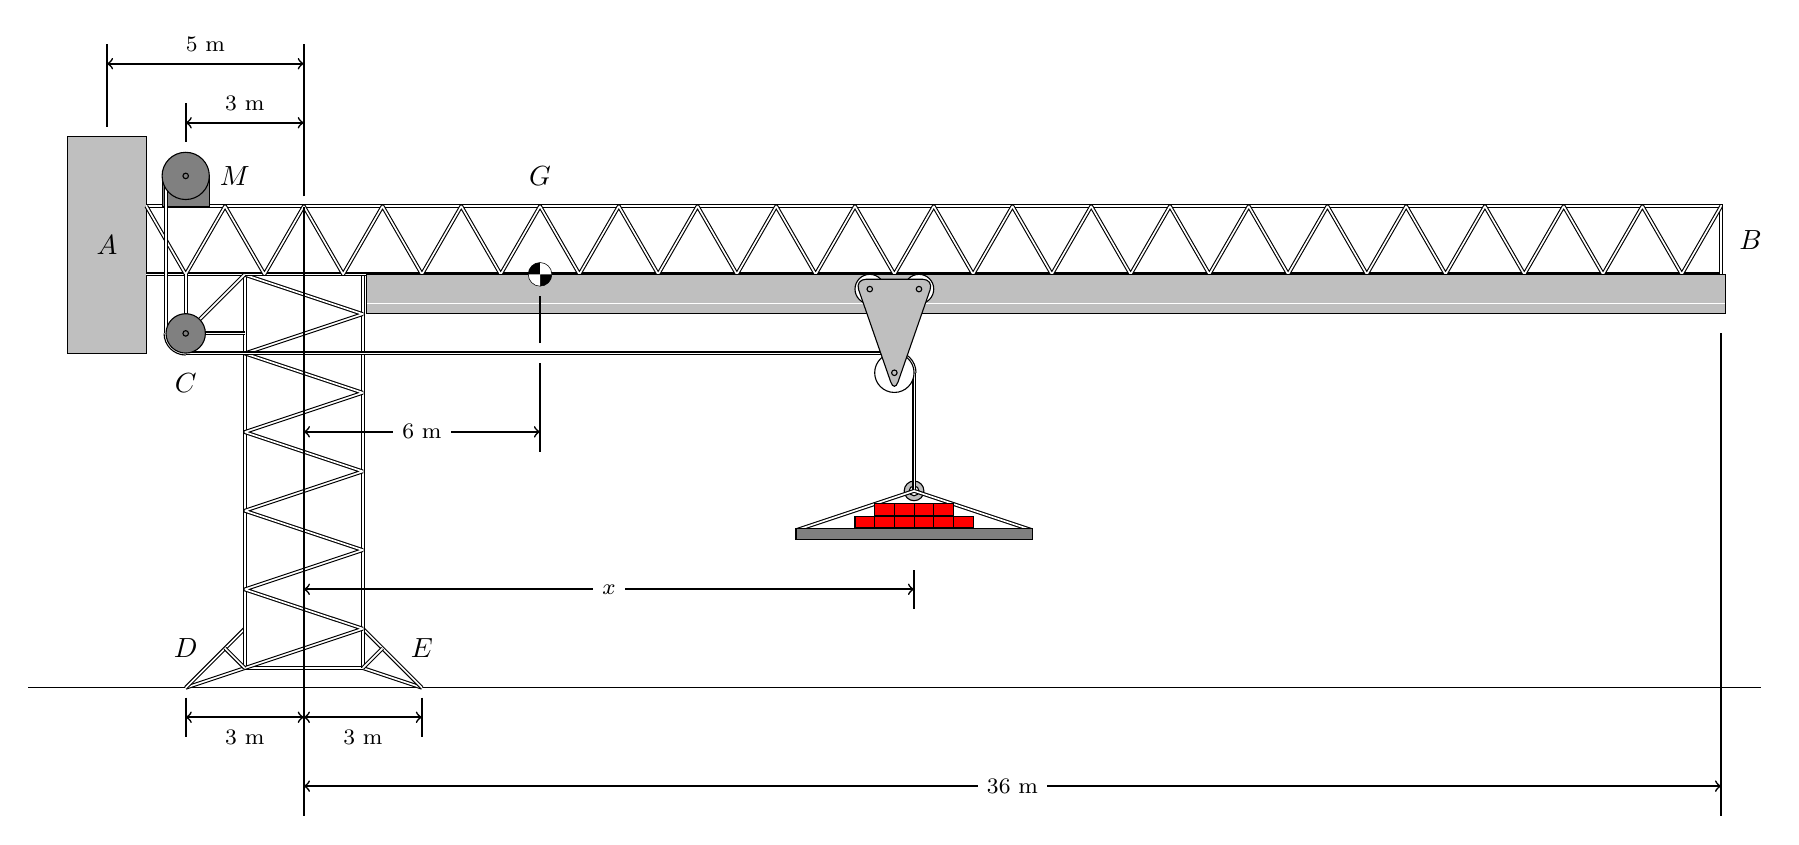
\begin{tikzpicture}[scale=0.5]
\draw (-4,0) -- (40,0);
\draw[double] (0,0) -- ++(1.5,0.5)--++(3,0)--++(1.5,-0.5);
\draw[double] (0,0) -- ++(1.5,1.5) ++(3,0)--++(1.5,-1.5);
\draw[double] (1.5,0.5) -- ++(0,10)--++(3,0)--++(0,-10);
\draw[double,join=bevel] (1.5,0.5) -- ++(18.43:3.16) -- ++(161.57:3.16) -- ++(18.43:3.16) -- ++(161.57:3.16) -- ++(18.43:3.16) -- ++(161.57:3.16) -- ++(18.43:3.16) -- ++(161.57:3.16) -- ++(18.43:3.16) -- ++(161.57:3.16);
\draw[double] (1.5,0.5) -- +(135:0.707);
\draw[double] (4.5,0.5) -- +(45:0.707);
\draw[fill=lightgray] (-1,8.5) rectangle (-3,14) node at +(1,-2.75) {$A$};
\draw[double] (-1,10.5) -- ++(40,0) -- ++(0,1.732) -- ++(-40,0);
\draw[double,join=bevel] (-1,10.5+1.732) -- ++(-60:2) -- ++(60:2) -- ++(-60:2) -- ++(60:2) -- ++(-60:2) -- ++(60:2) -- ++(-60:2) -- ++(60:2) -- ++(-60:2) -- ++(60:2) -- ++(-60:2) -- ++(60:2) -- ++(-60:2) -- ++(60:2) -- ++(-60:2) -- ++(60:2) -- ++(-60:2) -- ++(60:2) -- ++(-60:2) -- ++(60:2) -- ++(-60:2) -- ++(60:2) -- ++(-60:2) -- ++(60:2) -- ++(-60:2) -- ++(60:2) -- ++(-60:2) -- ++(60:2) -- ++(-60:2) -- ++(60:2) -- ++(-60:2) -- ++(60:2) -- ++(-60:2) -- ++(60:2) -- ++(-60:2) -- ++(60:2) -- ++(-60:2) -- ++(60:2) -- ++(-60:2) -- ++(60:2) node at +(0.75,-1.723/2) {$B$};
\draw[fill=lightgray] (4.6,10.5) rectangle (39.1,9.5);
\draw[double] (0,10.5) -- ++(0,-1.5) -- +(1.5,0);
\draw[double] (0,9) -- +(45:2.121);
\draw[fill=gray] (-0.6,13) rectangle (0.6,10.5+1.732);
\draw[fill=lightgray, even odd rule] (18.5,5) circle (0.25) circle (0.125);
\draw[double distance=0.4] (-0.5,13) -- ++(0,-4) ++(0.5,-0.5) -- ++(18,0) ++(0.5,-0.5) -- ++(0,-3);
\draw (18,8.55) arc (90:0:0.55);
\draw[fill=white] (18,8) circle (0.5);
\draw[color=white] (4.6,9.75) -- (39.1,9.75);
\draw[fill=white] (18.625,10.125) circle (0.375) +(-1.25,0) circle (0.375);
\draw[rounded corners, fill=lightgray] (18,7.5) -- (19,10.375) -- ++(-2,0) -- cycle;
\draw (18,8) circle (0.07);
\draw (18.625,10.125) circle (0.07) +(-1.25,0) circle (0.07);
\draw (-0.55,9) arc (180:270:0.55);
\draw[fill=gray] (0,9) circle (0.5) circle (0.07) node at +(0,-1.25) {$C$};
\draw[fill=gray] (0,13) circle (0.6) circle (0.07) node at +(1.25,0) {$M$};
\draw[double] (18.5,5) -- +(3,-1) (18.5,5) -- +(-3,-1);
\draw[fill=gray] (15.5,4.05) rectangle (21.5,3.755);
\draw[fill=red] (17,4.06) rectangle +(0.5,0.3);
\draw[fill=red] (17.5,4.06) rectangle +(0.5,0.3);
\draw[fill=red] (18,4.06) rectangle +(0.5,0.3);
\draw[fill=red] (18.5,4.06) rectangle +(0.5,0.3);
\draw[fill=red] (19,4.06) rectangle +(0.5,0.3);
\draw[fill=red] (19.5,4.06) rectangle +(0.5,0.3);
\draw[fill=red] (17.5,4.37) rectangle +(0.5,0.3);
\draw[fill=red] (18,4.37) rectangle +(0.5,0.3);
\draw[fill=red] (18.5,4.37) rectangle +(0.5,0.3);
\draw[fill=red] (19,4.37) rectangle +(0.5,0.3);
%Dimensions
\draw[semithick] (0,-0.25) -- +(0,-1) node at +(0,1.25) {$D$} ++(3,-3) -- +(0,3.25+10.5+1.723) ++(3,3) -- +(0,-1) node at +(0,1.25) {$E$} ++(33,-3) -- +(0,12.25);
\draw[semithick] (3,10.75+1.732) -- (3,13.6+0.25+1+1.5) ++(-3,-1.5) -- +(0,-1);
\draw[semithick] (-2,14.25) -- (-2,13.6+0.25+1+1.5);
\draw[semithick] (9,6)--++(0,2.25) ++(0,0.5)--(9,9.95);
\draw[semithick] (18.5,2) -- +(0,1);
\fill (9,10.5) -- ++(0.3,0) arc (0:-90:0.3) -- ++(0,0.6) arc (90:180:0.3);
\fill[white] (9,10.5) -- ++(0.3,0) arc (0:90:0.3) -- ++(0,-0.6) arc (270:180:0.3);
\draw[very thin] (9,10.5) circle (0.3) node at +(0,2.5) {$G$};
\draw[semithick, to-to] (0, -0.75) -- +(3,0) node[font=\footnotesize] at +(1.5,-0.5) {3 m};
\draw[semithick, to-to] (3, -0.75) -- +(3,0) node[font=\footnotesize] at +(1.5,-0.5) {3 m};
\draw[semithick, to-to] (3, -2.5) -- +(36,0) node[fill=white, font=\footnotesize] at +(18,0) {36 m};
\draw[semithick, to-to] (3,13.6+0.25+0.5) -- +(-3,0) node[font=\footnotesize] at +(-1.5,0.5) {3 m};
\draw[semithick, to-to] (3,13.6+0.25+2) -- +(-5,0) node[font=\footnotesize] at +(-2.5,0.5) {5 m};
\draw[semithick,to-to] (3,6.5) -- +(6,0) node[fill=white, font=\footnotesize] at +(3,0) {6 m};
\draw[semithick,to-to] (3,2.5) -- +(15.5,0) node[fill=white,font=\footnotesize] at +(7.75,0) {$x$};
\end{tikzpicture}
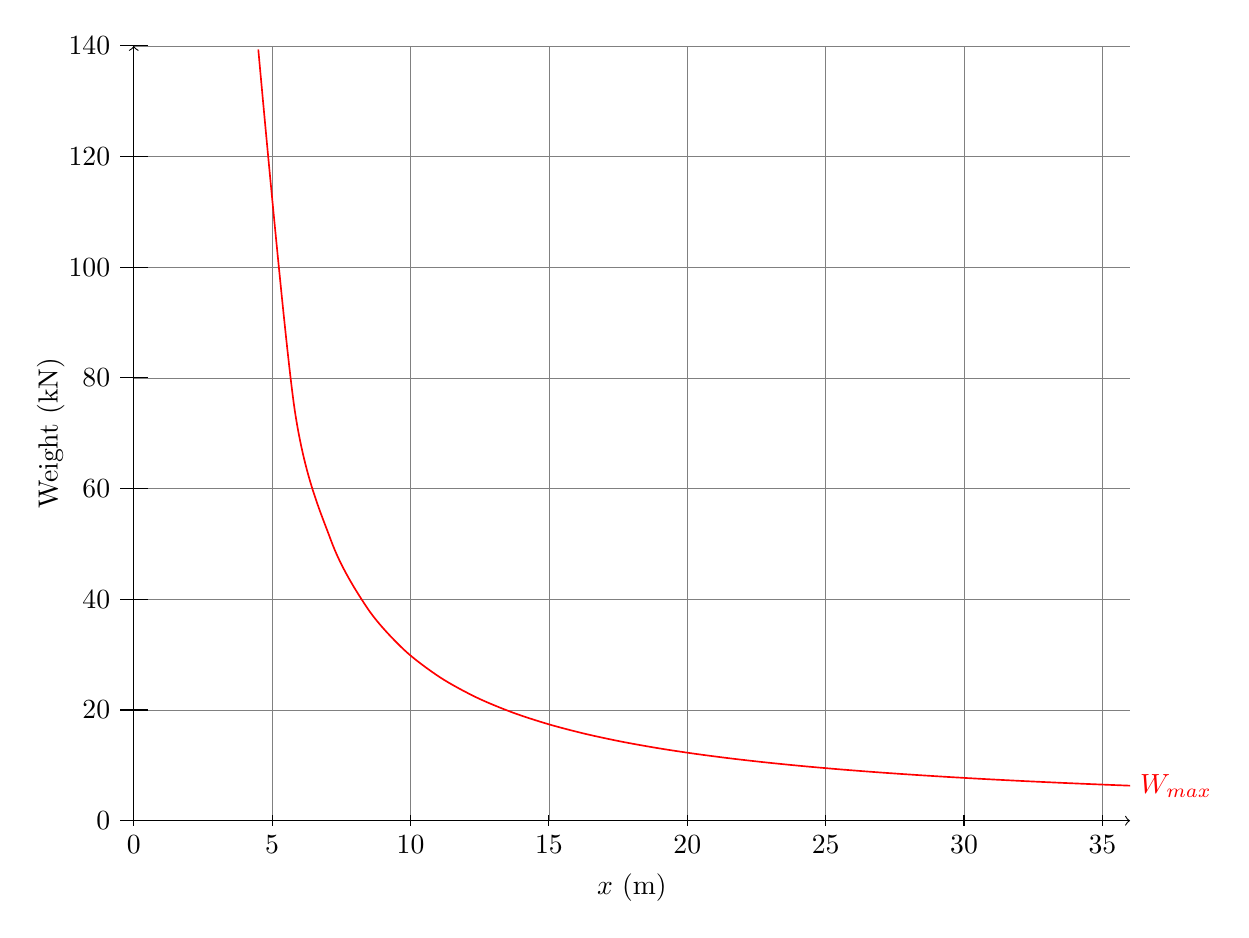
\begin{tikzpicture}[domain=0:36,x=100, y=20, scale=0.1]
    \draw[very thin,color=gray] (0,0) grid[xstep=5,ystep=20] (36,140);
    \foreach \x in {0,5,...,35}
        \draw (\x,1) -- (\x,-1)
            node[anchor=north] {\x};
\foreach \y in {0,20,...,140}
        \draw (0.5,\y) -- (-0.5,\y)
            node[anchor=east] {\y};
    \draw[->] (0,0) -- (36,0) node at +(-18,-12) {$x$ (m)}; 
    \draw[->] (0,0) -- (0,140) node[rotate=90] at +(-3,-70) {Weight (kN)};
    \draw[color=red,domain=4.5:36, smooth, semithick] plot (\x,{209/(\x-3)}) node[right] {$W_{max}$};
\end{tikzpicture}
\end{document}